\documentclass[10pt,a4paper]{article}
\usepackage[utf8]{inputenc}
\usepackage[T1]{fontenc}
\usepackage[french]{babel}
\usepackage{hyperref}
\usepackage{geometry}
\geometry{a4paper,margin=10mm,footskip=0mm}
%\setlength\leftmargin{2cm}
%\setlength\rightmargin{2cm}
\fontfamily{ppl}
\usepackage{graphicx}
\setlength\parindent{0pt}
\pagenumbering{gobble}
\frenchbsetup{StandardLists=true} % à inclure si on utilise \usepackage[french]{babel}
%\usepackage{enumitem}
\usepackage{amssymb}

\usepackage{soul}
\usepackage[svgnames]{xcolor}
\sethlcolor{LightYellow}
\newcommand{\grisclair}[1]{\colorbox{LightGray}{#1}}
%\newcommand{\bleupale}[1]{\colorbox{PaleTurquoise}{#1}}
\newcommand{\bleupale}[1]{\colorbox{AliceBlue}{#1}}

\title{\bfseries{SoCo : Formulaire d'inscription}}
%\author{Odile Bénassy}
\author{}
\date{}

\begin{document}
\pagestyle{empty}


\maketitle

\emph{Le formulaire SoCo d'inscription aux colloques s'utilise rapidement et facilite le travail d'organisation.}

\emph{Il est personnalisable.}

%\emph\small{NB: Il est d'un usage de plus en plus répandu d'éviter de privilégier un genre plutôt qu'un autre, mais nous tenons à préserver la qualité de la langue. En conséquence, pour le présent document, nous adoptons la convention suivante : nous parlerons d'un utilisateur - qui peut être aussi bien une utilisatrice bien évidemment - et d'une organisatrice - qui, de même, pourrait être aussi bien un organisateur.}

\section*{\bleupale{\emph{Liste des champs}}}

L'utilisateur est invité à remplir un petit nombre de champs : nom, prénom, adresse électronique, téléphone, fonction, organisation.

Seuls sont obligatoires : \emph{nom, prénom, organisation.}

En plus de cela, l'organisateu.rice peut demander d'autres informations, sous la forme de questions supplémentaires auxquelles l'utilisateur est alors invité à répondre (voir plus bas).

\section*{\bleupale{\emph{Composition du badge}}}

Le badge se compose sous ses yeux, sous la forme d'une première ligne comportant prénom et nom en majuscules, et une deuxième ligne avec fonction et organisation.

Dans l'intérêt d'une visibilité correcte des informations présentes sur le badge, une limite en nombre de caractères est instituée : 27 caractères pour la première lignes, 33 pour la deuxième (y compris les blancs ou tirets qui sont insérés). En cas de dépassement, le logiciel coupe le prénom ou la fonction. L'utilisateur peut corriger directement les lignes du badge avant soumission.

\begin{figure}[h]
  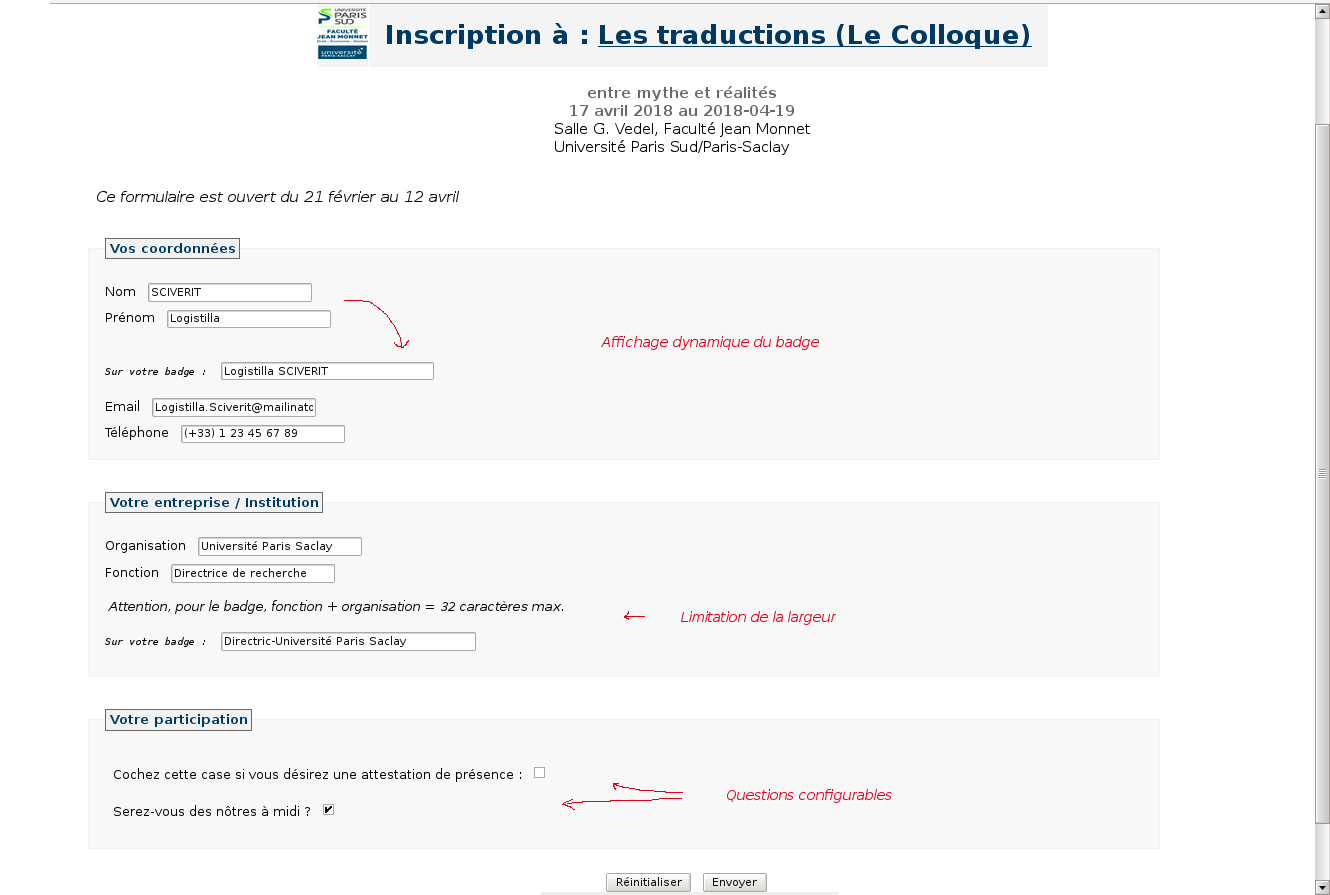
\includegraphics[width=500px]{images/formulaire-inscription-2}
\end{figure}

\newpage
\section*{\bleupale{\emph{Vérification de l'adresse}}}

L'adresse électronique est vérifiée :
\begin{itemize}
  \item Si l'adresse existe déjà dans la base (rare), ce n'est pas forcément un problème. Un message le signale sur la page.
  \item S'il s'agit de la même personne, alors le nom et le prénom fournis sur le formulaire doivent a priori correspondre à ce qui se trouve dans la base. Si ce n'est pas le cas, on envoie un message vers l'adresse mail en question, avec un code que l'utilisateur doit reporter dans une case du formulaire afin de se valider comme possesseur de cette adresse.
  \item Si le code fourni est le bon, on continue normalement le processus d'inscription mais le logiciel crée une nouvelle entrée, comme s'il s'agissait d'une nouvelle personne : puisque le nom ou le prénom sont modifiés, et pour éviter tout conflit avec d'éventuelles inscriptions antérieures, sur d'autres manifestations. Ce dispositif peut aussi permettre l'emploi de pseudonymes ou d'une autre présentation du nom ou du prénom, pour les cas de personnes mariées, ou tous autres cas que nous ne prévoyons pas forcément.
  \end{itemize}

\section*{\bleupale{\emph{Champs configurables}}}

Des questions supplémentaires peuvent être posées par les organisateu.rices : pour distinguer tel ou tel type d'inscription, statut, participation à des cocktails, commande d'actes...

Ces questions sont alors affichées à la suite des champs précédents.

\section*{\bleupale{\emph{Soumission}}}

Le formulaire SoCo tient sur une page unique. La soumission se fait très simplement, par pression sur le bouton ``Envoyer'', en bas de page.

Les champs sont vérifiés avant soumission définitive, et chaque champ obligatoire s'affiche bordé de rouge s'il n'est pas rempli.

%\section*{\bleupale{\emph{Améliorations prévues}}}

%Les améliorations suivantes sont en cours de développement :

%\begin{itemize}
%  \item Affichage d'un ``CAPTCHA'' pour décourager les robots
%  \item Solution d'affichage accessible aux malvoyants
%\end{itemize}

\vspace{1cm}
\fcolorbox{Black}{LightGray}{%
  \minipage[t]{\dimexpr0.9\linewidth-2\fboxsep-2\fboxrule\relax}
  \emph{Le logiciel SoCo a été réalisé, à l'UFR Jean Monnet de l'Université Paris Sud, par Odile Bénassy, responsable du service des systèmes d'information, en collaboration avec les responsables du service de la recherche du service de la communication. Ce logiciel prend la suite d'un autre, réalisé en 2007 par la même personne.}
  \endminipage}\hfill

%\fcolorbox{White}{White}{Fertig!}

\end{document}
